\chapter{Slow dynamics in colloidal supercooled liquids}
\label{ch:results_dynamics}

\section{Characterisation}
\label{sec:characterise_dyn}

\subsection{Two-Step relaxation}
\label{sec:result_2step}

We first have to confirm that our system actually displays the characteristic features of the dynamics of supercooled liquids. The coordinates tracked by confocal microscopy, linked to trajectories, which are analysed \latin{via} \EquationRef{eq:isf} and \EquationRef{eq:msd} to yield both the \ac{MSD} and the self \ac{ISF} as displayed in \FigureRef{fig:isf_msd}. For the calculation of the self \ac{ISF} we choose $q=2\pi/\sigma$. 

Times are scaled by the Brownian time $\tau_B=\unit{6.11}{\second}$, \latin{i.e.} the time needed for a single particle to diffuse over its own diameter at infinite dilution, and span nearly four decades. The curve of the most concentrated sample represents three days of acquisition, what means very close to our experimental $\phi_g$. For each volume fraction, the acquisition rate was set to catch the long term $\alpha$-relaxation, not the high frequency vibrations of the $\beta$-relaxation. We anyway see clearly the development of a plateau in both the correlation function and the diffusion.

\begin{figure}
	\centering
	\subfloat[Self \ac{ISF}]{\label{fig:isf}\resizebox{0.5\textwidth}{!}{\begin{Large}% GNUPLOT: LaTeX picture with Postscript
\begingroup
  \makeatletter
  \providecommand\color[2][]{%
    \GenericError{(gnuplot) \space\space\space\@spaces}{%
      Package color not loaded in conjunction with
      terminal option `colourtext'%
    }{See the gnuplot documentation for explanation.%
    }{Either use 'blacktext' in gnuplot or load the package
      color.sty in LaTeX.}%
    \renewcommand\color[2][]{}%
  }%
  \providecommand\includegraphics[2][]{%
    \GenericError{(gnuplot) \space\space\space\@spaces}{%
      Package graphicx or graphics not loaded%
    }{See the gnuplot documentation for explanation.%
    }{The gnuplot epslatex terminal needs graphicx.sty or graphics.sty.}%
    \renewcommand\includegraphics[2][]{}%
  }%
  \providecommand\rotatebox[2]{#2}%
  \@ifundefined{ifGPcolor}{%
    \newif\ifGPcolor
    \GPcolortrue
  }{}%
  \@ifundefined{ifGPblacktext}{%
    \newif\ifGPblacktext
    \GPblacktexttrue
  }{}%
  % define a \g@addto@macro without @ in the name:
  \let\gplgaddtomacro\g@addto@macro
  % define empty templates for all commands taking text:
  \gdef\gplbacktext{}%
  \gdef\gplfronttext{}%
  \makeatother
  \ifGPblacktext
    % no textcolor at all
    \def\colorrgb#1{}%
    \def\colorgray#1{}%
  \else
    % gray or color?
    \ifGPcolor
      \def\colorrgb#1{\color[rgb]{#1}}%
      \def\colorgray#1{\color[gray]{#1}}%
      \expandafter\def\csname LTw\endcsname{\color{white}}%
      \expandafter\def\csname LTb\endcsname{\color{black}}%
      \expandafter\def\csname LTa\endcsname{\color{black}}%
      \expandafter\def\csname LT0\endcsname{\color[rgb]{1,0,0}}%
      \expandafter\def\csname LT1\endcsname{\color[rgb]{0,1,0}}%
      \expandafter\def\csname LT2\endcsname{\color[rgb]{0,0,1}}%
      \expandafter\def\csname LT3\endcsname{\color[rgb]{1,0,1}}%
      \expandafter\def\csname LT4\endcsname{\color[rgb]{0,1,1}}%
      \expandafter\def\csname LT5\endcsname{\color[rgb]{1,1,0}}%
      \expandafter\def\csname LT6\endcsname{\color[rgb]{0,0,0}}%
      \expandafter\def\csname LT7\endcsname{\color[rgb]{1,0.3,0}}%
      \expandafter\def\csname LT8\endcsname{\color[rgb]{0.5,0.5,0.5}}%
    \else
      % gray
      \def\colorrgb#1{\color{black}}%
      \def\colorgray#1{\color[gray]{#1}}%
      \expandafter\def\csname LTw\endcsname{\color{white}}%
      \expandafter\def\csname LTb\endcsname{\color{black}}%
      \expandafter\def\csname LTa\endcsname{\color{black}}%
      \expandafter\def\csname LT0\endcsname{\color{black}}%
      \expandafter\def\csname LT1\endcsname{\color{black}}%
      \expandafter\def\csname LT2\endcsname{\color{black}}%
      \expandafter\def\csname LT3\endcsname{\color{black}}%
      \expandafter\def\csname LT4\endcsname{\color{black}}%
      \expandafter\def\csname LT5\endcsname{\color{black}}%
      \expandafter\def\csname LT6\endcsname{\color{black}}%
      \expandafter\def\csname LT7\endcsname{\color{black}}%
      \expandafter\def\csname LT8\endcsname{\color{black}}%
    \fi
  \fi
  \setlength{\unitlength}{0.0500bp}%
  \begin{picture}(7200.00,5040.00)%
    \gplgaddtomacro\gplbacktext{%
      \csname LTb\endcsname%
      \put(1056,1518){\makebox(0,0)[r]{\strut{}$0.2$}}%
      \put(1056,2333){\makebox(0,0)[r]{\strut{}$0.4$}}%
      \put(1056,3147){\makebox(0,0)[r]{\strut{}$0.6$}}%
      \put(1056,3962){\makebox(0,0)[r]{\strut{}$0.8$}}%
      \put(1056,4776){\makebox(0,0)[r]{\strut{}$1$}}%
      \put(1251,484){\makebox(0,0){\strut{}$10^{0}$}}%
      \put(2628,484){\makebox(0,0){\strut{}$10^{1}$}}%
      \put(4006,484){\makebox(0,0){\strut{}$10^{2}$}}%
      \put(5383,484){\makebox(0,0){\strut{}$10^{3}$}}%
      \put(6760,484){\makebox(0,0){\strut{}$10^{4}$}}%
      \put(418,2740){\rotatebox{-270}{\makebox(0,0){\strut{}Self \ac{ISF}}}}%
      \put(6979,2740){\rotatebox{-270}{\makebox(0,0){\strut{}}}}%
      \put(3974,154){\makebox(0,0){\strut{}$t/\tau_B$}}%
      \put(3974,4666){\makebox(0,0){\strut{}}}%
      \put(3974,4665){\makebox(0,0){\strut{}}}%
      \put(264,110){\makebox(0,0)[l]{\strut{}}}%
    }%
    \gplgaddtomacro\gplfronttext{%
      \csname LTb\endcsname%
      \put(6037,3525){\makebox(0,0)[r]{\strut{}$\phi=0.497$}}%
      \csname LTb\endcsname%
      \put(6037,3789){\makebox(0,0)[r]{\strut{}$\phi=0.535$}}%
      \csname LTb\endcsname%
      \put(6037,4053){\makebox(0,0)[r]{\strut{}$\phi=0.540$}}%
      \csname LTb\endcsname%
      \put(6037,4317){\makebox(0,0)[r]{\strut{}$\phi=0.555$}}%
      \csname LTb\endcsname%
      \put(6037,4581){\makebox(0,0)[r]{\strut{}$\phi=0.576$}}%
    }%
    \gplbacktext
    \put(0,0){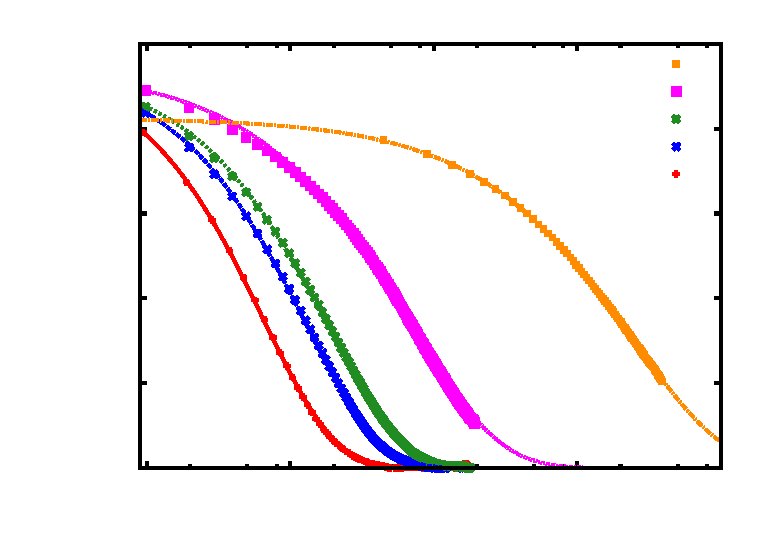
\includegraphics{./fit_isf}}%
    \gplfronttext
  \end{picture}%
\endgroup
\end{Large}}}
	\subfloat[\ac{MSD}]{\label{fig:msd}\resizebox{0.5\textwidth}{!}{\begin{Large}% GNUPLOT: LaTeX picture with Postscript
\begingroup
  \makeatletter
  \providecommand\color[2][]{%
    \GenericError{(gnuplot) \space\space\space\@spaces}{%
      Package color not loaded in conjunction with
      terminal option `colourtext'%
    }{See the gnuplot documentation for explanation.%
    }{Either use 'blacktext' in gnuplot or load the package
      color.sty in LaTeX.}%
    \renewcommand\color[2][]{}%
  }%
  \providecommand\includegraphics[2][]{%
    \GenericError{(gnuplot) \space\space\space\@spaces}{%
      Package graphicx or graphics not loaded%
    }{See the gnuplot documentation for explanation.%
    }{The gnuplot epslatex terminal needs graphicx.sty or graphics.sty.}%
    \renewcommand\includegraphics[2][]{}%
  }%
  \providecommand\rotatebox[2]{#2}%
  \@ifundefined{ifGPcolor}{%
    \newif\ifGPcolor
    \GPcolortrue
  }{}%
  \@ifundefined{ifGPblacktext}{%
    \newif\ifGPblacktext
    \GPblacktexttrue
  }{}%
  % define a \g@addto@macro without @ in the name:
  \let\gplgaddtomacro\g@addto@macro
  % define empty templates for all commands taking text:
  \gdef\gplbacktext{}%
  \gdef\gplfronttext{}%
  \makeatother
  \ifGPblacktext
    % no textcolor at all
    \def\colorrgb#1{}%
    \def\colorgray#1{}%
  \else
    % gray or color?
    \ifGPcolor
      \def\colorrgb#1{\color[rgb]{#1}}%
      \def\colorgray#1{\color[gray]{#1}}%
      \expandafter\def\csname LTw\endcsname{\color{white}}%
      \expandafter\def\csname LTb\endcsname{\color{black}}%
      \expandafter\def\csname LTa\endcsname{\color{black}}%
      \expandafter\def\csname LT0\endcsname{\color[rgb]{1,0,0}}%
      \expandafter\def\csname LT1\endcsname{\color[rgb]{0,1,0}}%
      \expandafter\def\csname LT2\endcsname{\color[rgb]{0,0,1}}%
      \expandafter\def\csname LT3\endcsname{\color[rgb]{1,0,1}}%
      \expandafter\def\csname LT4\endcsname{\color[rgb]{0,1,1}}%
      \expandafter\def\csname LT5\endcsname{\color[rgb]{1,1,0}}%
      \expandafter\def\csname LT6\endcsname{\color[rgb]{0,0,0}}%
      \expandafter\def\csname LT7\endcsname{\color[rgb]{1,0.3,0}}%
      \expandafter\def\csname LT8\endcsname{\color[rgb]{0.5,0.5,0.5}}%
    \else
      % gray
      \def\colorrgb#1{\color{black}}%
      \def\colorgray#1{\color[gray]{#1}}%
      \expandafter\def\csname LTw\endcsname{\color{white}}%
      \expandafter\def\csname LTb\endcsname{\color{black}}%
      \expandafter\def\csname LTa\endcsname{\color{black}}%
      \expandafter\def\csname LT0\endcsname{\color{black}}%
      \expandafter\def\csname LT1\endcsname{\color{black}}%
      \expandafter\def\csname LT2\endcsname{\color{black}}%
      \expandafter\def\csname LT3\endcsname{\color{black}}%
      \expandafter\def\csname LT4\endcsname{\color{black}}%
      \expandafter\def\csname LT5\endcsname{\color{black}}%
      \expandafter\def\csname LT6\endcsname{\color{black}}%
      \expandafter\def\csname LT7\endcsname{\color{black}}%
      \expandafter\def\csname LT8\endcsname{\color{black}}%
    \fi
  \fi
  \setlength{\unitlength}{0.0500bp}%
  \begin{picture}(7200.00,5040.00)%
    \gplgaddtomacro\gplbacktext{%
      \csname LTb\endcsname%
      \put(1056,704){\makebox(0,0)[r]{\strut{}$10^{-2}$}}%
      \put(1056,2061){\makebox(0,0)[r]{\strut{}$10^{-1}$}}%
      \put(1056,3419){\makebox(0,0)[r]{\strut{}$10^{0}$}}%
      \put(1056,4776){\makebox(0,0)[r]{\strut{}$10^{1}$}}%
      \put(1251,484){\makebox(0,0){\strut{}$10^{0}$}}%
      \put(2628,484){\makebox(0,0){\strut{}$10^{1}$}}%
      \put(4006,484){\makebox(0,0){\strut{}$10^{2}$}}%
      \put(5383,484){\makebox(0,0){\strut{}$10^{3}$}}%
      \put(6760,484){\makebox(0,0){\strut{}$10^{4}$}}%
      \put(286,2740){\rotatebox{-270}{\makebox(0,0){\strut{}$\Delta r^2/\sigma^2$}}}%
      \put(6979,2740){\rotatebox{-270}{\makebox(0,0){\strut{}}}}%
      \put(3974,154){\makebox(0,0){\strut{}$t/\tau_B$}}%
      \put(3974,4666){\makebox(0,0){\strut{}}}%
      \put(3974,4665){\makebox(0,0){\strut{}}}%
      \put(-264,110){\makebox(0,0)[l]{\strut{}}}%
    }%
    \gplgaddtomacro\gplfronttext{%
      \csname LTb\endcsname%
      \put(2904,4581){\makebox(0,0)[r]{\strut{}$\phi=0.497$}}%
      \csname LTb\endcsname%
      \put(2904,4317){\makebox(0,0)[r]{\strut{}$\phi=0.535$}}%
      \csname LTb\endcsname%
      \put(2904,4053){\makebox(0,0)[r]{\strut{}$\phi=0.540$}}%
      \csname LTb\endcsname%
      \put(2904,3789){\makebox(0,0)[r]{\strut{}$\phi=0.555$}}%
      \csname LTb\endcsname%
      \put(2904,3525){\makebox(0,0)[r]{\strut{}$\phi=0.576$}}%
    }%
    \gplbacktext
    \put(0,0){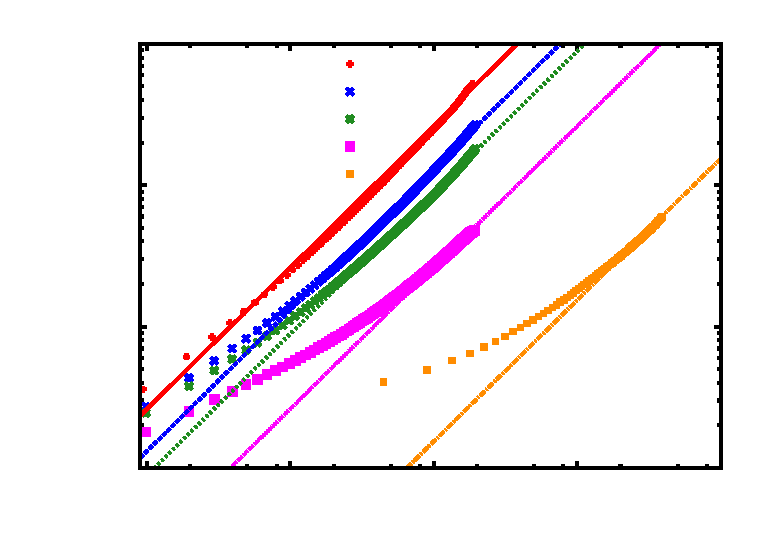
\includegraphics{./fit_msd}}%
    \gplfronttext
  \end{picture}%
\endgroup
\end{Large}}}
	\caption{Overall dynamics of our system calculated from the tracked coordinates, for various volume fractions. The lines are least square fits by \EquationRef{eq:streched_exp} in~\subref{fig:isf} and by the long term diffusion $\Delta r^2 = 6 D t$ in~\subref{fig:msd}.}
	\label{fig:isf_msd}
\end{figure}

We are able to fit the self \ac{ISF} at each volume fraction by a stretched exponential
\begin{equation}
	F_s(q,t\gg\tau_\beta) \sim A \exp{\left[ -\left( \frac{t}{\tau_\alpha} \right)^\beta\right] }
	\label{eq:streched_exp}
\end{equation}
which is the long time part of \EquationRef{eq:streched_exp_2steps}. To get a nice fit of the short times, where the errors are mostly averaged out, and because our data are equally separated in linear time while the decay spans orders of magnitude, we weighted the points by $1/\log(t)^2$. As expected, the height of the plateau $A$ and the stretching exponent $\beta$ do not depend strongly on the volume fraction even if slightly decreasing with increasing $\phi$. However the relaxation time $\tau_\alpha$ is (as expected) strongly dependent on $\phi$ (see \FigureRef{fig:fit_vft}).

\begin{figure}
	\centering
	\subfloat
		[Volume fraction dependence of $\tau_\alpha$ and $t^{dh}$.]
		{\label{fig:fit_vft}\resizebox{0.5\textwidth}{!}{\begin{Large}% GNUPLOT: LaTeX picture with Postscript
\begingroup
  \makeatletter
  \providecommand\color[2][]{%
    \GenericError{(gnuplot) \space\space\space\@spaces}{%
      Package color not loaded in conjunction with
      terminal option `colourtext'%
    }{See the gnuplot documentation for explanation.%
    }{Either use 'blacktext' in gnuplot or load the package
      color.sty in LaTeX.}%
    \renewcommand\color[2][]{}%
  }%
  \providecommand\includegraphics[2][]{%
    \GenericError{(gnuplot) \space\space\space\@spaces}{%
      Package graphicx or graphics not loaded%
    }{See the gnuplot documentation for explanation.%
    }{The gnuplot epslatex terminal needs graphicx.sty or graphics.sty.}%
    \renewcommand\includegraphics[2][]{}%
  }%
  \providecommand\rotatebox[2]{#2}%
  \@ifundefined{ifGPcolor}{%
    \newif\ifGPcolor
    \GPcolortrue
  }{}%
  \@ifundefined{ifGPblacktext}{%
    \newif\ifGPblacktext
    \GPblacktexttrue
  }{}%
  % define a \g@addto@macro without @ in the name:
  \let\gplgaddtomacro\g@addto@macro
  % define empty templates for all commands taking text:
  \gdef\gplbacktext{}%
  \gdef\gplfronttext{}%
  \makeatother
  \ifGPblacktext
    % no textcolor at all
    \def\colorrgb#1{}%
    \def\colorgray#1{}%
  \else
    % gray or color?
    \ifGPcolor
      \def\colorrgb#1{\color[rgb]{#1}}%
      \def\colorgray#1{\color[gray]{#1}}%
      \expandafter\def\csname LTw\endcsname{\color{white}}%
      \expandafter\def\csname LTb\endcsname{\color{black}}%
      \expandafter\def\csname LTa\endcsname{\color{black}}%
      \expandafter\def\csname LT0\endcsname{\color[rgb]{1,0,0}}%
      \expandafter\def\csname LT1\endcsname{\color[rgb]{0,1,0}}%
      \expandafter\def\csname LT2\endcsname{\color[rgb]{0,0,1}}%
      \expandafter\def\csname LT3\endcsname{\color[rgb]{1,0,1}}%
      \expandafter\def\csname LT4\endcsname{\color[rgb]{0,1,1}}%
      \expandafter\def\csname LT5\endcsname{\color[rgb]{1,1,0}}%
      \expandafter\def\csname LT6\endcsname{\color[rgb]{0,0,0}}%
      \expandafter\def\csname LT7\endcsname{\color[rgb]{1,0.3,0}}%
      \expandafter\def\csname LT8\endcsname{\color[rgb]{0.5,0.5,0.5}}%
    \else
      % gray
      \def\colorrgb#1{\color{black}}%
      \def\colorgray#1{\color[gray]{#1}}%
      \expandafter\def\csname LTw\endcsname{\color{white}}%
      \expandafter\def\csname LTb\endcsname{\color{black}}%
      \expandafter\def\csname LTa\endcsname{\color{black}}%
      \expandafter\def\csname LT0\endcsname{\color{black}}%
      \expandafter\def\csname LT1\endcsname{\color{black}}%
      \expandafter\def\csname LT2\endcsname{\color{black}}%
      \expandafter\def\csname LT3\endcsname{\color{black}}%
      \expandafter\def\csname LT4\endcsname{\color{black}}%
      \expandafter\def\csname LT5\endcsname{\color{black}}%
      \expandafter\def\csname LT6\endcsname{\color{black}}%
      \expandafter\def\csname LT7\endcsname{\color{black}}%
      \expandafter\def\csname LT8\endcsname{\color{black}}%
    \fi
  \fi
  \setlength{\unitlength}{0.0500bp}%
  \begin{picture}(7200.00,5040.00)%
    \gplgaddtomacro\gplbacktext{%
      \csname LTb\endcsname%
      \put(1056,704){\makebox(0,0)[r]{\strut{}$10^{0}$}}%
      \put(1056,1722){\makebox(0,0)[r]{\strut{}$10^{1}$}}%
      \put(1056,2740){\makebox(0,0)[r]{\strut{}$10^{2}$}}%
      \put(1056,3758){\makebox(0,0)[r]{\strut{}$10^{3}$}}%
      \put(1056,4776){\makebox(0,0)[r]{\strut{}$10^{4}$}}%
      \put(1967,484){\makebox(0,0){\strut{}$0.50$}}%
      \put(3165,484){\makebox(0,0){\strut{}$0.52$}}%
      \put(4363,484){\makebox(0,0){\strut{}$0.54$}}%
      \put(5562,484){\makebox(0,0){\strut{}$0.56$}}%
      \put(6760,484){\makebox(0,0){\strut{}$0.58$}}%
      \put(418,2740){\rotatebox{-270}{\makebox(0,0){\strut{}$t/\tau_B$}}}%
      \put(6979,2740){\rotatebox{-270}{\makebox(0,0){\strut{}}}}%
      \put(3974,154){\makebox(0,0){\strut{}$\phi$}}%
      \put(3974,4666){\makebox(0,0){\strut{}}}%
      \put(3974,4665){\makebox(0,0){\strut{}}}%
      \put(-132,110){\makebox(0,0)[l]{\strut{}}}%
    }%
    \gplgaddtomacro\gplfronttext{%
      \csname LTb\endcsname%
      \put(4620,4556){\makebox(0,0)[r]{\strut{}$\tau_\alpha$ experiments}}%
      \csname LTb\endcsname%
      \put(4620,4241){\makebox(0,0)[r]{\strut{}$\tau_\alpha$ simulations}}%
      \csname LTb\endcsname%
      \put(4620,3926){\makebox(0,0)[r]{\strut{}$t^{dh}$ experiments}}%
      \csname LTb\endcsname%
      \put(4620,3611){\makebox(0,0)[r]{\strut{}$t^{dh}$ simulations}}%
    }%
    \gplbacktext
    \put(0,0){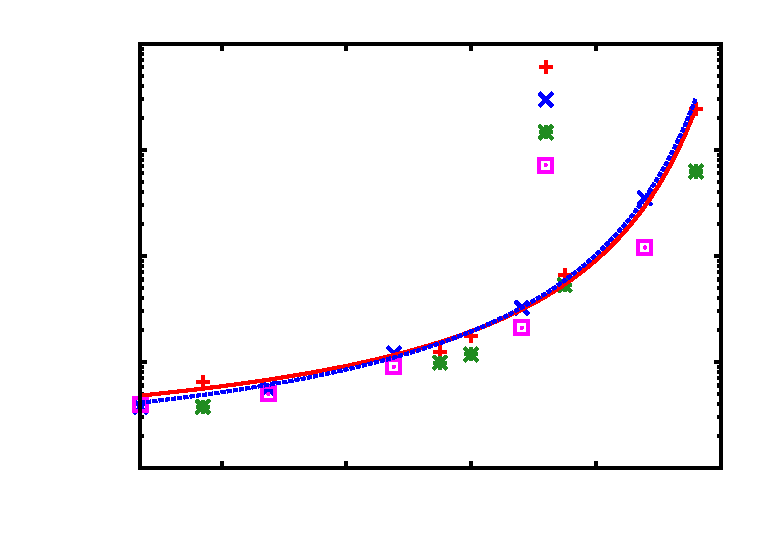
\includegraphics{fit_vft}}%
    \gplfronttext
  \end{picture}%
\endgroup
\end{Large}}}
	\subfloat
		[Evolution of the \ac{NGP} with supercooling.]
		{\label{fig:ngp}\resizebox{0.5\textwidth}{!}{\begin{Large}% GNUPLOT: LaTeX picture with Postscript
\begingroup
  \makeatletter
  \providecommand\color[2][]{%
    \GenericError{(gnuplot) \space\space\space\@spaces}{%
      Package color not loaded in conjunction with
      terminal option `colourtext'%
    }{See the gnuplot documentation for explanation.%
    }{Either use 'blacktext' in gnuplot or load the package
      color.sty in LaTeX.}%
    \renewcommand\color[2][]{}%
  }%
  \providecommand\includegraphics[2][]{%
    \GenericError{(gnuplot) \space\space\space\@spaces}{%
      Package graphicx or graphics not loaded%
    }{See the gnuplot documentation for explanation.%
    }{The gnuplot epslatex terminal needs graphicx.sty or graphics.sty.}%
    \renewcommand\includegraphics[2][]{}%
  }%
  \providecommand\rotatebox[2]{#2}%
  \@ifundefined{ifGPcolor}{%
    \newif\ifGPcolor
    \GPcolortrue
  }{}%
  \@ifundefined{ifGPblacktext}{%
    \newif\ifGPblacktext
    \GPblacktexttrue
  }{}%
  % define a \g@addto@macro without @ in the name:
  \let\gplgaddtomacro\g@addto@macro
  % define empty templates for all commands taking text:
  \gdef\gplbacktext{}%
  \gdef\gplfronttext{}%
  \makeatother
  \ifGPblacktext
    % no textcolor at all
    \def\colorrgb#1{}%
    \def\colorgray#1{}%
  \else
    % gray or color?
    \ifGPcolor
      \def\colorrgb#1{\color[rgb]{#1}}%
      \def\colorgray#1{\color[gray]{#1}}%
      \expandafter\def\csname LTw\endcsname{\color{white}}%
      \expandafter\def\csname LTb\endcsname{\color{black}}%
      \expandafter\def\csname LTa\endcsname{\color{black}}%
      \expandafter\def\csname LT0\endcsname{\color[rgb]{1,0,0}}%
      \expandafter\def\csname LT1\endcsname{\color[rgb]{0,1,0}}%
      \expandafter\def\csname LT2\endcsname{\color[rgb]{0,0,1}}%
      \expandafter\def\csname LT3\endcsname{\color[rgb]{1,0,1}}%
      \expandafter\def\csname LT4\endcsname{\color[rgb]{0,1,1}}%
      \expandafter\def\csname LT5\endcsname{\color[rgb]{1,1,0}}%
      \expandafter\def\csname LT6\endcsname{\color[rgb]{0,0,0}}%
      \expandafter\def\csname LT7\endcsname{\color[rgb]{1,0.3,0}}%
      \expandafter\def\csname LT8\endcsname{\color[rgb]{0.5,0.5,0.5}}%
    \else
      % gray
      \def\colorrgb#1{\color{black}}%
      \def\colorgray#1{\color[gray]{#1}}%
      \expandafter\def\csname LTw\endcsname{\color{white}}%
      \expandafter\def\csname LTb\endcsname{\color{black}}%
      \expandafter\def\csname LTa\endcsname{\color{black}}%
      \expandafter\def\csname LT0\endcsname{\color{black}}%
      \expandafter\def\csname LT1\endcsname{\color{black}}%
      \expandafter\def\csname LT2\endcsname{\color{black}}%
      \expandafter\def\csname LT3\endcsname{\color{black}}%
      \expandafter\def\csname LT4\endcsname{\color{black}}%
      \expandafter\def\csname LT5\endcsname{\color{black}}%
      \expandafter\def\csname LT6\endcsname{\color{black}}%
      \expandafter\def\csname LT7\endcsname{\color{black}}%
      \expandafter\def\csname LT8\endcsname{\color{black}}%
    \fi
  \fi
  \setlength{\unitlength}{0.0500bp}%
  \begin{picture}(7200.00,5040.00)%
    \gplgaddtomacro\gplbacktext{%
      \csname LTb\endcsname%
      \put(1056,704){\makebox(0,0)[r]{\strut{}$0$}}%
      \put(1056,1213){\makebox(0,0)[r]{\strut{}$0.2$}}%
      \put(1056,1722){\makebox(0,0)[r]{\strut{}$0.4$}}%
      \put(1056,2231){\makebox(0,0)[r]{\strut{}$0.6$}}%
      \put(1056,2740){\makebox(0,0)[r]{\strut{}$0.8$}}%
      \put(1056,3249){\makebox(0,0)[r]{\strut{}$1$}}%
      \put(1056,3758){\makebox(0,0)[r]{\strut{}$1.2$}}%
      \put(1056,4267){\makebox(0,0)[r]{\strut{}$1.4$}}%
      \put(1056,4776){\makebox(0,0)[r]{\strut{}$1.6$}}%
      \put(1251,484){\makebox(0,0){\strut{}$10^{0}$}}%
      \put(2628,484){\makebox(0,0){\strut{}$10^{1}$}}%
      \put(4006,484){\makebox(0,0){\strut{}$10^{2}$}}%
      \put(5383,484){\makebox(0,0){\strut{}$10^{3}$}}%
      \put(6760,484){\makebox(0,0){\strut{}$10^{4}$}}%
      \put(418,2740){\rotatebox{-270}{\makebox(0,0){\strut{}Non gaussian parameter}}}%
      \put(6979,2740){\rotatebox{-270}{\makebox(0,0){\strut{}}}}%
      \put(3974,154){\makebox(0,0){\strut{}$t/\tau_B$}}%
      \put(3974,4666){\makebox(0,0){\strut{}}}%
      \put(3974,4665){\makebox(0,0){\strut{}}}%
      \put(264,110){\makebox(0,0)[l]{\strut{}}}%
    }%
    \gplgaddtomacro\gplfronttext{%
      \csname LTb\endcsname%
      \put(2904,3228){\makebox(0,0)[r]{\strut{}$\phi=0.497$}}%
      \csname LTb\endcsname%
      \put(2904,3558){\makebox(0,0)[r]{\strut{}$\phi=0.535$}}%
      \csname LTb\endcsname%
      \put(2904,3888){\makebox(0,0)[r]{\strut{}$\phi=0.540$}}%
      \csname LTb\endcsname%
      \put(2904,4218){\makebox(0,0)[r]{\strut{}$\phi=0.555$}}%
      \csname LTb\endcsname%
      \put(2904,4548){\makebox(0,0)[r]{\strut{}$\phi=0.576$}}%
    }%
    \gplbacktext
    \put(0,0){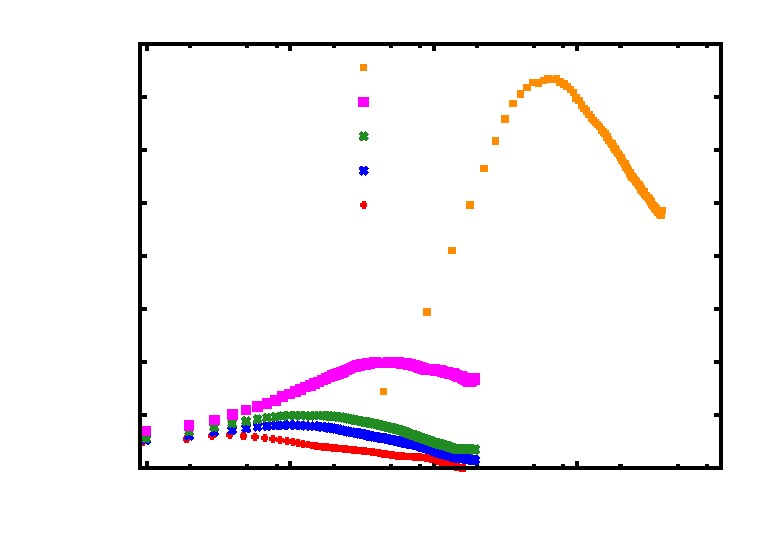
\includegraphics{fit_ngp}}%
    \gplfronttext
  \end{picture}%
\endgroup
\end{Large}}}
	\caption{The curves in \subref{fig:fit_vft} are the fits of the respective relaxation times $\tau_\alpha$ by the \acs{VFT} law.}
	\label{fig:vtf_ngp}
\end{figure}

We were able to fit the volume fraction dependence of $\tau_\alpha$ by the \ac{VFT} law (see \EquationRef{eq:VFT}) which yield a fragility of $\mathcal{D}^{exp} = 0.280$ and $\phi_0^{exp}=0.597$. Kasasaki's simulations results are plotted on the same graph and are in good agreement even if an independent fit yield slightly different values $\mathcal{D}^{sim} = 0.380$ and $\phi_0^{sim}=0.603$.

We check that our system actually displays non-Gaussian dynamics by calculating the \ac{NGP} (see \EquationRef{eq:ngp}). As expected, we observe the bell shape growing and shifting toward longer times with supercooling (see \FigureRef{fig:ngp}). Our samples actually have the two populations of mobile and localised particles described in \SectionRef{sec:nongaussian}. The decrease of the \ac{NGP} at long times is observed even in our densest sample, confirming its ergodicity. The time lags $t^{dh}$ corresponding to the maximum of the \ac{NGP} are reported on \FigureRef{fig:fit_vft}.

\subsection{Dynamic Heterogeneities}
\label{sec:result_dynhet}

Following \citet{weeks2000}, we display the dynamic heterogeneities by plotting the $10\%$ fastest particles in \FigureRef{fig:dh_3d}, where the displacements are calculated between the displayed configuration $t_0$ and $t_0+t^{dh}$. Visually, the characteristic length scale of the dynamic heterogeneities grows with the supercooling.

\begin{figure}
	\centering
	\begin{small}%
	\tikz\shade[ball color=white] circle (0.4em);
	Isolated\qquad%
	\tikz\shade[ball color=blue] circle (0.4em);%
	\tikz\shade[ball color=green] circle (0.4em);%
	\tikz\shade[ball color=orange] circle (0.4em);%
	\tikz\shade[ball color=red] circle (0.4em);
	Connected%
	\end{small}\\
	\subfloat[Normal liquid ($\phi=0.497$)]{
		\label{fig:dh_3d_liq}
		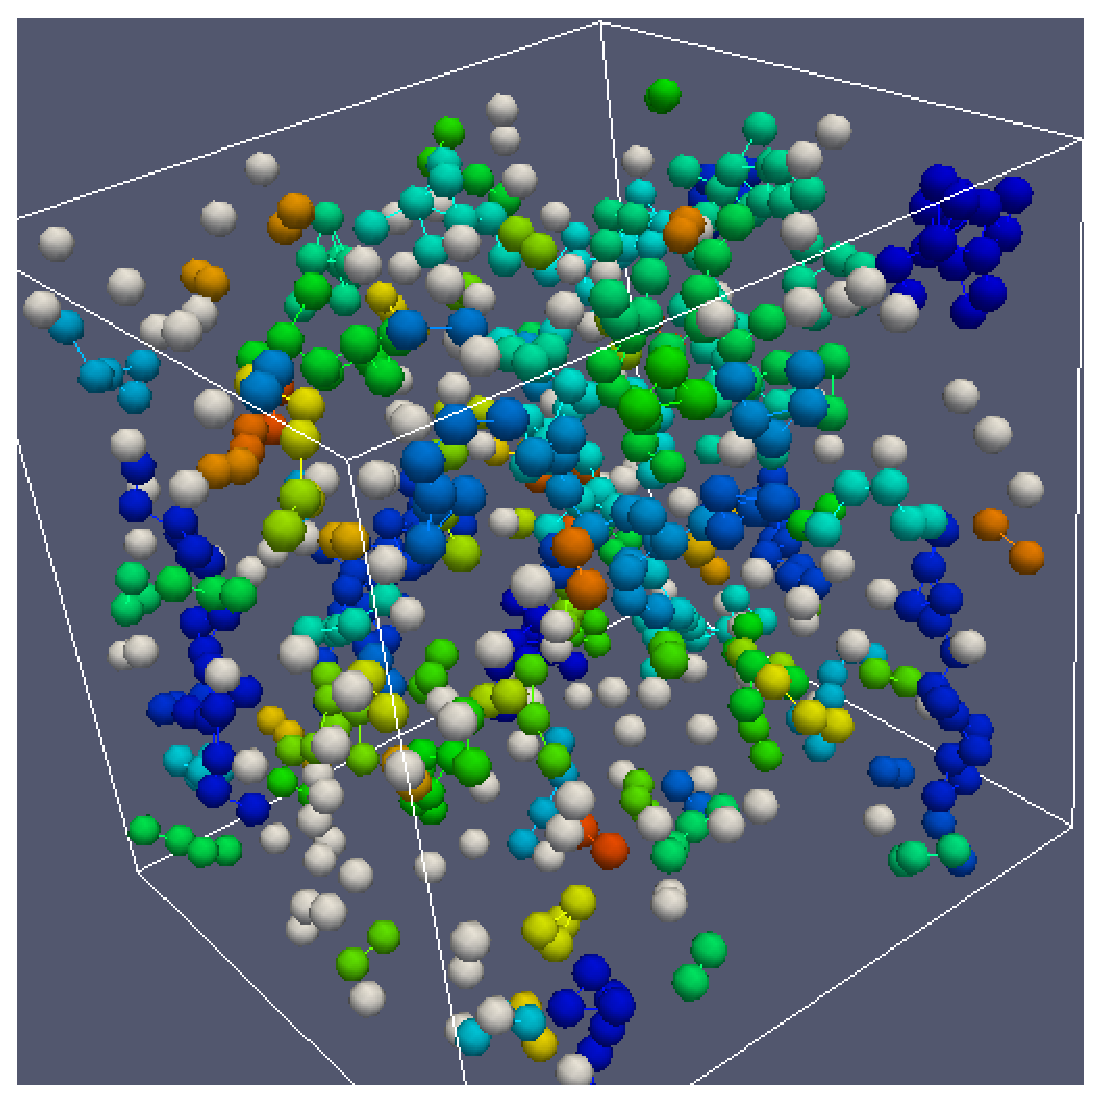
\includegraphics[width=0.4\textwidth]{dh_3954}}\quad
	\subfloat[Supercooled liquid ($\phi=0.535$)]{
		\label{fig:dh_3d_sc}
		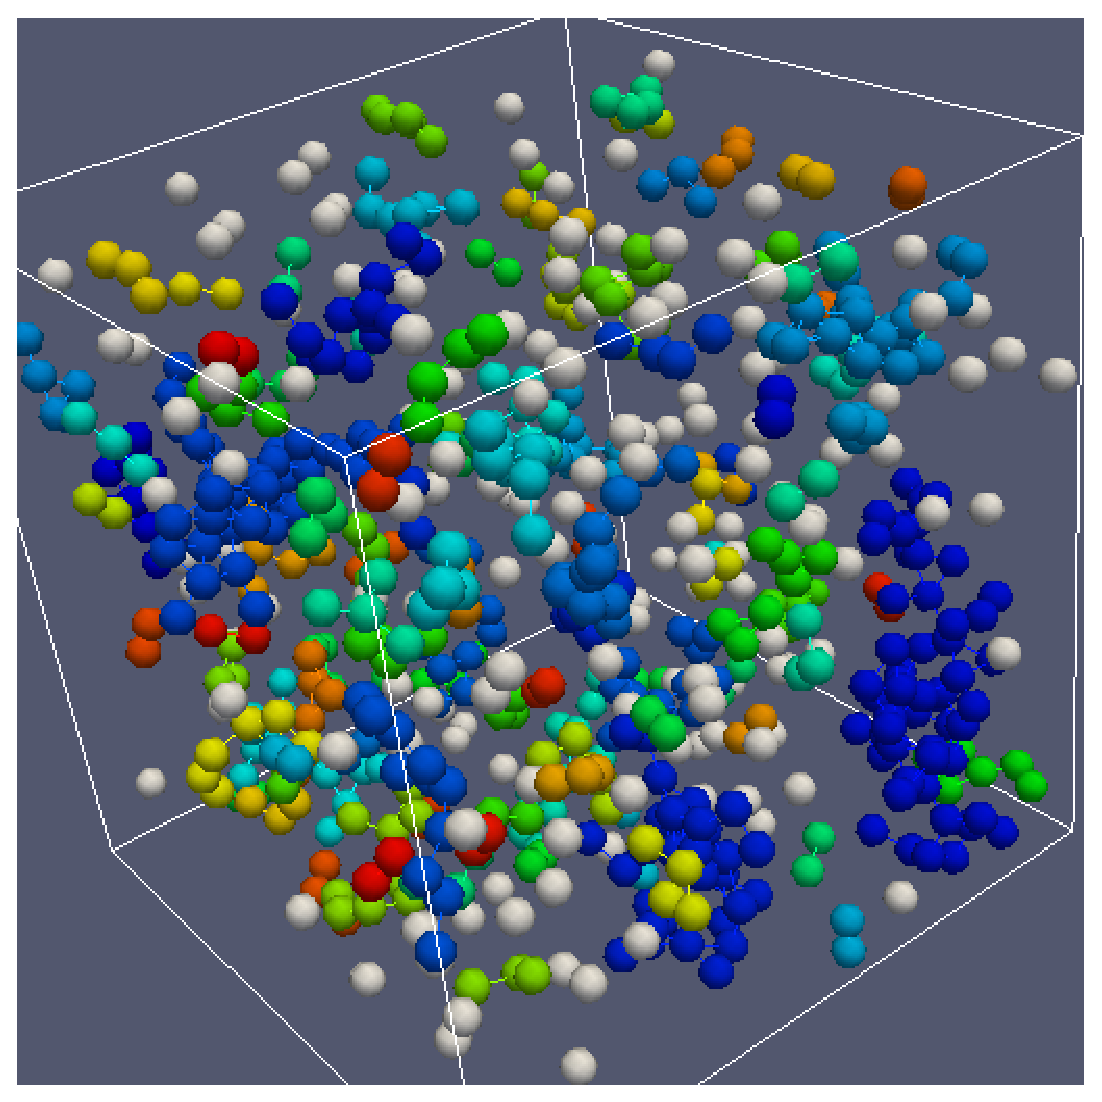
\includegraphics[width=0.4\textwidth]{dh_4582}}
	\caption{$10\%$ fastest particles. Neighbouring particles are displayed with the same colour.}
\end{figure}
\begin{figure}
	\ContinuedFloat
	\centering
	\begin{small}%
	\tikz\shade[ball color=white] circle (0.4em);
	Isolated\qquad%
	\tikz\shade[ball color=blue] circle (0.4em);%
	\tikz\shade[ball color=green] circle (0.4em);%
	\tikz\shade[ball color=orange] circle (0.4em);%
	\tikz\shade[ball color=red] circle (0.4em);
	Connected%
	\end{small}\\
	\subfloat
		[Deeply supercooled ($\phi=0.576$). We are looking through a slice of the sample of thickness $\sim 8 \sigma$.]{
		\label{fig:dh_3d_deep}
		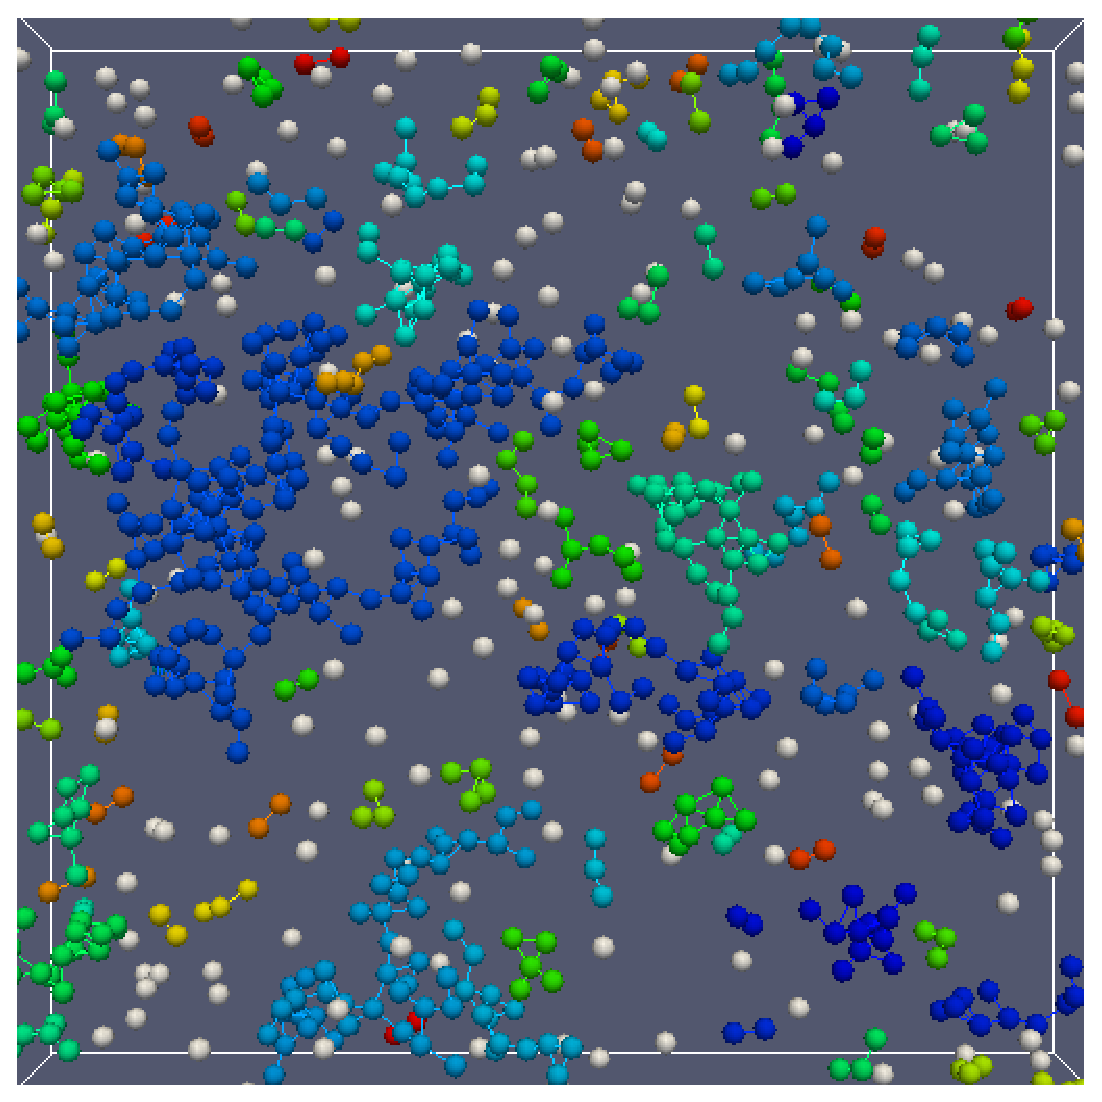
\includegraphics[width=0.8\textwidth]{dh_go1}}
	\caption{Computer reconstruction from confocal microscopy coordinates. Only the $10\%$ fastest particles (see text) are displayed for clarity. The colours differentiate between disconnected clusters of fast particles. White particles are isolated fast particles.}
	\label{fig:dh_3d}
\end{figure}

To be more quantitative, we compute the mobility-mobility correlation function $\mathcal{G}_u(r,t)$ (defined in \EquationRef{eq:mobility_correl}) for $t=t^{dh}$. As shown in \FigureRef{fig:G_u}, the correlation is longer and longer ranged with increasing the volume fraction. We characterise the decay of the correlation by fitting the upper envelope of $\mathcal{G}_u(r,t^{dh})$ by the Ornstein-Zernike function (see \EquationRef{eq:OZ}).

\begin{figure}
	\centering
	\subfloat
		[Mobility-mobility spatial correlation.]
		{\label{fig:G_u}\resizebox{0.5\textwidth}{!}{\begin{Large}% GNUPLOT: LaTeX picture with Postscript
\begingroup
  \makeatletter
  \providecommand\color[2][]{%
    \GenericError{(gnuplot) \space\space\space\@spaces}{%
      Package color not loaded in conjunction with
      terminal option `colourtext'%
    }{See the gnuplot documentation for explanation.%
    }{Either use 'blacktext' in gnuplot or load the package
      color.sty in LaTeX.}%
    \renewcommand\color[2][]{}%
  }%
  \providecommand\includegraphics[2][]{%
    \GenericError{(gnuplot) \space\space\space\@spaces}{%
      Package graphicx or graphics not loaded%
    }{See the gnuplot documentation for explanation.%
    }{The gnuplot epslatex terminal needs graphicx.sty or graphics.sty.}%
    \renewcommand\includegraphics[2][]{}%
  }%
  \providecommand\rotatebox[2]{#2}%
  \@ifundefined{ifGPcolor}{%
    \newif\ifGPcolor
    \GPcolortrue
  }{}%
  \@ifundefined{ifGPblacktext}{%
    \newif\ifGPblacktext
    \GPblacktexttrue
  }{}%
  % define a \g@addto@macro without @ in the name:
  \let\gplgaddtomacro\g@addto@macro
  % define empty templates for all commands taking text:
  \gdef\gplbacktext{}%
  \gdef\gplfronttext{}%
  \makeatother
  \ifGPblacktext
    % no textcolor at all
    \def\colorrgb#1{}%
    \def\colorgray#1{}%
  \else
    % gray or color?
    \ifGPcolor
      \def\colorrgb#1{\color[rgb]{#1}}%
      \def\colorgray#1{\color[gray]{#1}}%
      \expandafter\def\csname LTw\endcsname{\color{white}}%
      \expandafter\def\csname LTb\endcsname{\color{black}}%
      \expandafter\def\csname LTa\endcsname{\color{black}}%
      \expandafter\def\csname LT0\endcsname{\color[rgb]{1,0,0}}%
      \expandafter\def\csname LT1\endcsname{\color[rgb]{0,1,0}}%
      \expandafter\def\csname LT2\endcsname{\color[rgb]{0,0,1}}%
      \expandafter\def\csname LT3\endcsname{\color[rgb]{1,0,1}}%
      \expandafter\def\csname LT4\endcsname{\color[rgb]{0,1,1}}%
      \expandafter\def\csname LT5\endcsname{\color[rgb]{1,1,0}}%
      \expandafter\def\csname LT6\endcsname{\color[rgb]{0,0,0}}%
      \expandafter\def\csname LT7\endcsname{\color[rgb]{1,0.3,0}}%
      \expandafter\def\csname LT8\endcsname{\color[rgb]{0.5,0.5,0.5}}%
    \else
      % gray
      \def\colorrgb#1{\color{black}}%
      \def\colorgray#1{\color[gray]{#1}}%
      \expandafter\def\csname LTw\endcsname{\color{white}}%
      \expandafter\def\csname LTb\endcsname{\color{black}}%
      \expandafter\def\csname LTa\endcsname{\color{black}}%
      \expandafter\def\csname LT0\endcsname{\color{black}}%
      \expandafter\def\csname LT1\endcsname{\color{black}}%
      \expandafter\def\csname LT2\endcsname{\color{black}}%
      \expandafter\def\csname LT3\endcsname{\color{black}}%
      \expandafter\def\csname LT4\endcsname{\color{black}}%
      \expandafter\def\csname LT5\endcsname{\color{black}}%
      \expandafter\def\csname LT6\endcsname{\color{black}}%
      \expandafter\def\csname LT7\endcsname{\color{black}}%
      \expandafter\def\csname LT8\endcsname{\color{black}}%
    \fi
  \fi
  \setlength{\unitlength}{0.0500bp}%
  \begin{picture}(7200.00,5040.00)%
    \gplgaddtomacro\gplbacktext{%
      \csname LTb\endcsname%
      \put(1056,704){\makebox(0,0)[r]{\strut{}$10^{-4}$}}%
      \put(1056,1938){\makebox(0,0)[r]{\strut{}$10^{-3}$}}%
      \put(1056,3171){\makebox(0,0)[r]{\strut{}$10^{-2}$}}%
      \put(1056,4405){\makebox(0,0)[r]{\strut{}$10^{-1}$}}%
      \put(1368,484){\makebox(0,0){\strut{}$2$}}%
      \put(2266,484){\makebox(0,0){\strut{}$3$}}%
      \put(3165,484){\makebox(0,0){\strut{}$4$}}%
      \put(4064,484){\makebox(0,0){\strut{}$5$}}%
      \put(4963,484){\makebox(0,0){\strut{}$6$}}%
      \put(5861,484){\makebox(0,0){\strut{}$7$}}%
      \put(6760,484){\makebox(0,0){\strut{}$8$}}%
      \put(286,2740){\rotatebox{-270}{\makebox(0,0){\strut{}$\mathcal{G}_u(r,t^{dh})/\Delta r^2(t^{dh})$}}}%
      \put(6979,2740){\rotatebox{-270}{\makebox(0,0){\strut{}}}}%
      \put(3974,154){\makebox(0,0){\strut{}$r/\sigma$}}%
      \put(3974,4666){\makebox(0,0){\strut{}}}%
      \put(3974,4665){\makebox(0,0){\strut{}}}%
      \put(-264,110){\makebox(0,0)[l]{\strut{}}}%
    }%
    \gplgaddtomacro\gplfronttext{%
      \csname LTb\endcsname%
      \put(2904,932){\makebox(0,0)[r]{\strut{}$\phi=0.497$}}%
      \csname LTb\endcsname%
      \put(2904,1262){\makebox(0,0)[r]{\strut{}$\phi=0.555$}}%
      \csname LTb\endcsname%
      \put(2904,1592){\makebox(0,0)[r]{\strut{}$\phi=0.576$}}%
    }%
    \gplbacktext
    \put(0,0){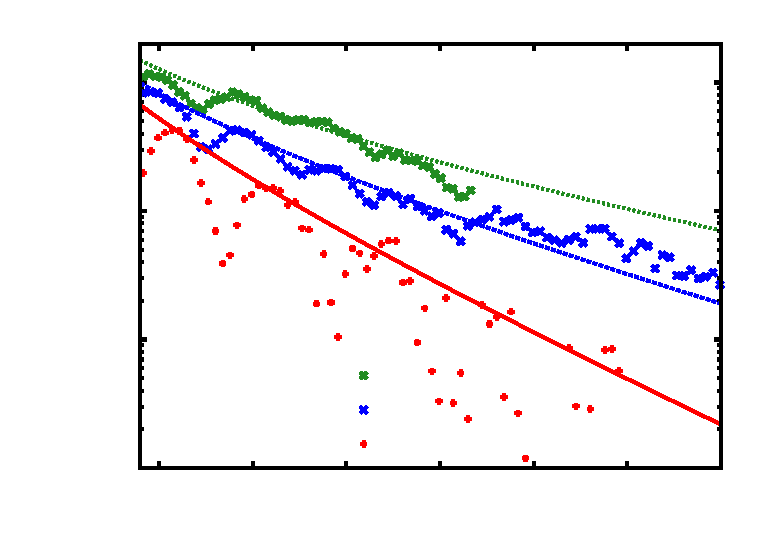
\includegraphics{fit_gu}}%
    \gplfronttext
  \end{picture}%
\endgroup
\end{Large}}}
	\subfloat
		[Volume fraction dependence of the correlation lengths.]{\label{fig:fit_xi}\resizebox{0.5\textwidth}{!}{\begin{Large}% GNUPLOT: LaTeX picture with Postscript
\begingroup
  \makeatletter
  \providecommand\color[2][]{%
    \GenericError{(gnuplot) \space\space\space\@spaces}{%
      Package color not loaded in conjunction with
      terminal option `colourtext'%
    }{See the gnuplot documentation for explanation.%
    }{Either use 'blacktext' in gnuplot or load the package
      color.sty in LaTeX.}%
    \renewcommand\color[2][]{}%
  }%
  \providecommand\includegraphics[2][]{%
    \GenericError{(gnuplot) \space\space\space\@spaces}{%
      Package graphicx or graphics not loaded%
    }{See the gnuplot documentation for explanation.%
    }{The gnuplot epslatex terminal needs graphicx.sty or graphics.sty.}%
    \renewcommand\includegraphics[2][]{}%
  }%
  \providecommand\rotatebox[2]{#2}%
  \@ifundefined{ifGPcolor}{%
    \newif\ifGPcolor
    \GPcolortrue
  }{}%
  \@ifundefined{ifGPblacktext}{%
    \newif\ifGPblacktext
    \GPblacktexttrue
  }{}%
  % define a \g@addto@macro without @ in the name:
  \let\gplgaddtomacro\g@addto@macro
  % define empty templates for all commands taking text:
  \gdef\gplbacktext{}%
  \gdef\gplfronttext{}%
  \makeatother
  \ifGPblacktext
    % no textcolor at all
    \def\colorrgb#1{}%
    \def\colorgray#1{}%
  \else
    % gray or color?
    \ifGPcolor
      \def\colorrgb#1{\color[rgb]{#1}}%
      \def\colorgray#1{\color[gray]{#1}}%
      \expandafter\def\csname LTw\endcsname{\color{white}}%
      \expandafter\def\csname LTb\endcsname{\color{black}}%
      \expandafter\def\csname LTa\endcsname{\color{black}}%
      \expandafter\def\csname LT0\endcsname{\color[rgb]{1,0,0}}%
      \expandafter\def\csname LT1\endcsname{\color[rgb]{0,1,0}}%
      \expandafter\def\csname LT2\endcsname{\color[rgb]{0,0,1}}%
      \expandafter\def\csname LT3\endcsname{\color[rgb]{1,0,1}}%
      \expandafter\def\csname LT4\endcsname{\color[rgb]{0,1,1}}%
      \expandafter\def\csname LT5\endcsname{\color[rgb]{1,1,0}}%
      \expandafter\def\csname LT6\endcsname{\color[rgb]{0,0,0}}%
      \expandafter\def\csname LT7\endcsname{\color[rgb]{1,0.3,0}}%
      \expandafter\def\csname LT8\endcsname{\color[rgb]{0.5,0.5,0.5}}%
    \else
      % gray
      \def\colorrgb#1{\color{black}}%
      \def\colorgray#1{\color[gray]{#1}}%
      \expandafter\def\csname LTw\endcsname{\color{white}}%
      \expandafter\def\csname LTb\endcsname{\color{black}}%
      \expandafter\def\csname LTa\endcsname{\color{black}}%
      \expandafter\def\csname LT0\endcsname{\color{black}}%
      \expandafter\def\csname LT1\endcsname{\color{black}}%
      \expandafter\def\csname LT2\endcsname{\color{black}}%
      \expandafter\def\csname LT3\endcsname{\color{black}}%
      \expandafter\def\csname LT4\endcsname{\color{black}}%
      \expandafter\def\csname LT5\endcsname{\color{black}}%
      \expandafter\def\csname LT6\endcsname{\color{black}}%
      \expandafter\def\csname LT7\endcsname{\color{black}}%
      \expandafter\def\csname LT8\endcsname{\color{black}}%
    \fi
  \fi
  \setlength{\unitlength}{0.0500bp}%
  \begin{picture}(7200.00,5040.00)%
    \gplgaddtomacro\gplbacktext{%
      \csname LTb\endcsname%
      \put(792,704){\makebox(0,0)[r]{\strut{}$0$}}%
      \put(792,1609){\makebox(0,0)[r]{\strut{}$1$}}%
      \put(792,2514){\makebox(0,0)[r]{\strut{}$2$}}%
      \put(792,3419){\makebox(0,0)[r]{\strut{}$3$}}%
      \put(792,4324){\makebox(0,0)[r]{\strut{}$4$}}%
      \put(1572,484){\makebox(0,0){\strut{}$0.5$}}%
      \put(2869,484){\makebox(0,0){\strut{}$0.52$}}%
      \put(4166,484){\makebox(0,0){\strut{}$0.54$}}%
      \put(5463,484){\makebox(0,0){\strut{}$0.56$}}%
      \put(6760,484){\makebox(0,0){\strut{}$0.58$}}%
      \put(418,2740){\rotatebox{-270}{\makebox(0,0){\strut{}$\xi/\sigma$}}}%
      \put(6979,2740){\rotatebox{-270}{\makebox(0,0){\strut{}}}}%
      \put(3842,154){\makebox(0,0){\strut{}$\phi$}}%
      \put(3842,4666){\makebox(0,0){\strut{}}}%
      \put(3842,4665){\makebox(0,0){\strut{}}}%
      \put(264,110){\makebox(0,0)[l]{\strut{}}}%
    }%
    \gplgaddtomacro\gplfronttext{%
      \csname LTb\endcsname%
      \put(3432,4556){\makebox(0,0)[r]{\strut{}Dynamical $\xi_u$}}%
      \csname LTb\endcsname%
      \put(3432,4241){\makebox(0,0)[r]{\strut{}Structural $\xi_6$}}%
    }%
    \gplbacktext
    \put(0,0){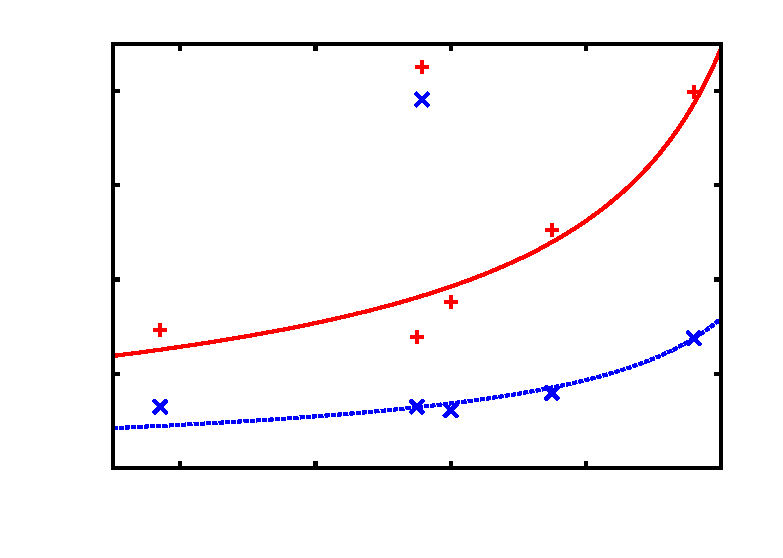
\includegraphics{fit_xi}}%
    \gplfronttext
  \end{picture}%
\endgroup
\end{Large}}}
	\caption{Spatial correlation of the dynamic heterogeneities. The lines in \subref{fig:G_u} are the fit by the Ornstein-Zernike function (see \EquationRef{eq:OZ}). The lines in \subref{fig:fit_xi} are power-law fit (see \EquationRef{eq:xi_power}).}
	\label{fig:dh_fit}
\end{figure}

The volume fraction dependence of the dynamic correlation length $\xi_u$ resulting from the previous fit can be well described by a power-law divergence at $\phi_0$ (see \FigureRef{fig:fit_xi}):
\begin{equation}
	\xi(\phi) \propto \xi_0 \left( \frac{\phi_0 - \phi}{\phi} \right)^{-\frac{2}{3}}
	\label{eq:xi_power}
\end{equation}
where $\phi_0=\phi_0^{exp}$ is set by the \ac{VFT} fit of the relaxation times (see \SectionRef{sec:result_2step}). The only adjustable parameter is the value of $\xi_0$. This result is in perfect agreement with \citet{tanaka2010critical} and suggest that the dynamical heterogeneities in hard spheres are the manifestation of critical fluctuations. We note that the exponent of this power law is the same as the critical exponent for the d-dimensional Ising universality class within errors: $\nu = (2-\alpha)/d$, with $\alpha \simeq 0.1$ in 3D and thus $\nu \simeq 0.63$~\cite{onuki, Chaikin2000}, close to our exponent of $-2/3$.

\section{Link between structure and dynamics}
\label{sec:struct_vs_dyn}

As stated in \SectionRef{sec:static_cause} we will now try to explain the dynamic heterogeneities by a purely static cause, \latin{i.e.} the structural heterogeneities observed in \ChapterRef{ch:structure}.

\subsection{Correlation lengths}
\label{sec:correlation_lengths}

The first piece of the answer comes following \citet{tanaka2010critical}: the correlation length of the crystal-like bond order $\xi_6$ that we calculated in \SectionRef{sec:mrco_spatial} diverges at $\phi_0$ following the same power law as $\xi_u$, as displayed in \FigureRef{fig:fit_xi}. This indicates a strong link between the fluctuations of the crystal-like bond order and the dynamic heterogeneities, probably of a critical nature.

However, the role of the icosahedral order remains unclear, especially at shallow supercooling were the aforementioned power-law fit is not perfect and the icosahedra the majority structure.

\subsection{Where are the fast particles?}

In \FigureRef{fig:proportions_phi} we plot the proportion of the $10\%$ fastest particles amongst crystal-like bond ordered ($Q_6>Q_6^{mrco}$) particles, icosahedral ($w_6<w_6^{dodec}$) particles and perfect icosahedra ($w_6<w_6^*$). There are clearly fewer fast particles amongst the strongly bond ordered particles than in the bulk. However, the proportion of fast particles in the imperfect icosahedral network is not significantly different from the bulk. We also check the number of fast particles amongst the non-icosahedral particles that are neighbours of icosahedra, but once again, the proportion is the same as in the overall population

\begin{figure}
	\centering
	\resizebox{0.8\textwidth}{!}{% GNUPLOT: LaTeX picture with Postscript
\begingroup
  \makeatletter
  \providecommand\color[2][]{%
    \GenericError{(gnuplot) \space\space\space\@spaces}{%
      Package color not loaded in conjunction with
      terminal option `colourtext'%
    }{See the gnuplot documentation for explanation.%
    }{Either use 'blacktext' in gnuplot or load the package
      color.sty in LaTeX.}%
    \renewcommand\color[2][]{}%
  }%
  \providecommand\includegraphics[2][]{%
    \GenericError{(gnuplot) \space\space\space\@spaces}{%
      Package graphicx or graphics not loaded%
    }{See the gnuplot documentation for explanation.%
    }{The gnuplot epslatex terminal needs graphicx.sty or graphics.sty.}%
    \renewcommand\includegraphics[2][]{}%
  }%
  \providecommand\rotatebox[2]{#2}%
  \@ifundefined{ifGPcolor}{%
    \newif\ifGPcolor
    \GPcolortrue
  }{}%
  \@ifundefined{ifGPblacktext}{%
    \newif\ifGPblacktext
    \GPblacktexttrue
  }{}%
  % define a \g@addto@macro without @ in the name:
  \let\gplgaddtomacro\g@addto@macro
  % define empty templates for all commands taking text:
  \gdef\gplbacktext{}%
  \gdef\gplfronttext{}%
  \makeatother
  \ifGPblacktext
    % no textcolor at all
    \def\colorrgb#1{}%
    \def\colorgray#1{}%
  \else
    % gray or color?
    \ifGPcolor
      \def\colorrgb#1{\color[rgb]{#1}}%
      \def\colorgray#1{\color[gray]{#1}}%
      \expandafter\def\csname LTw\endcsname{\color{white}}%
      \expandafter\def\csname LTb\endcsname{\color{black}}%
      \expandafter\def\csname LTa\endcsname{\color{black}}%
      \expandafter\def\csname LT0\endcsname{\color[rgb]{1,0,0}}%
      \expandafter\def\csname LT1\endcsname{\color[rgb]{0,1,0}}%
      \expandafter\def\csname LT2\endcsname{\color[rgb]{0,0,1}}%
      \expandafter\def\csname LT3\endcsname{\color[rgb]{1,0,1}}%
      \expandafter\def\csname LT4\endcsname{\color[rgb]{0,1,1}}%
      \expandafter\def\csname LT5\endcsname{\color[rgb]{1,1,0}}%
      \expandafter\def\csname LT6\endcsname{\color[rgb]{0,0,0}}%
      \expandafter\def\csname LT7\endcsname{\color[rgb]{1,0.3,0}}%
      \expandafter\def\csname LT8\endcsname{\color[rgb]{0.5,0.5,0.5}}%
    \else
      % gray
      \def\colorrgb#1{\color{black}}%
      \def\colorgray#1{\color[gray]{#1}}%
      \expandafter\def\csname LTw\endcsname{\color{white}}%
      \expandafter\def\csname LTb\endcsname{\color{black}}%
      \expandafter\def\csname LTa\endcsname{\color{black}}%
      \expandafter\def\csname LT0\endcsname{\color{black}}%
      \expandafter\def\csname LT1\endcsname{\color{black}}%
      \expandafter\def\csname LT2\endcsname{\color{black}}%
      \expandafter\def\csname LT3\endcsname{\color{black}}%
      \expandafter\def\csname LT4\endcsname{\color{black}}%
      \expandafter\def\csname LT5\endcsname{\color{black}}%
      \expandafter\def\csname LT6\endcsname{\color{black}}%
      \expandafter\def\csname LT7\endcsname{\color{black}}%
      \expandafter\def\csname LT8\endcsname{\color{black}}%
    \fi
  \fi
  \setlength{\unitlength}{0.0500bp}%
  \begin{picture}(7200.00,5040.00)%
    \gplgaddtomacro\gplbacktext{%
      \csname LTb\endcsname%
      \put(1254,699){\makebox(0,0)[r]{\strut{}$0.00$}}%
      \put(1254,1718){\makebox(0,0)[r]{\strut{}$0.05$}}%
      \put(1254,2738){\makebox(0,0)[r]{\strut{}$0.10$}}%
      \put(1254,3757){\makebox(0,0)[r]{\strut{}$0.15$}}%
      \put(1254,4776){\makebox(0,0)[r]{\strut{}$0.20$}}%
      \put(2228,484){\makebox(0,0){\strut{}$0.51$}}%
      \put(3523,484){\makebox(0,0){\strut{}$0.53$}}%
      \put(4818,484){\makebox(0,0){\strut{}$0.55$}}%
      \put(6113,484){\makebox(0,0){\strut{}$0.57$}}%
      \put(484,2740){\rotatebox{90}{\makebox(0,0){\strut{}Proportion of the 10\% fastest particles}}}%
      \put(6979,2740){\rotatebox{90}{\makebox(0,0){\strut{}}}}%
      \put(4073,154){\makebox(0,0){\strut{}$\phi$}}%
      \put(4073,4666){\makebox(0,0){\strut{}}}%
      \put(4073,4665){\makebox(0,0){\strut{}}}%
      \put(330,110){\makebox(0,0)[l]{\strut{}}}%
    }%
    \gplgaddtomacro\gplfronttext{%
      \csname LTb\endcsname%
      \put(4422,4556){\makebox(0,0)[r]{\strut{}in Crystal-like}}%
      \csname LTb\endcsname%
      \put(4422,4241){\makebox(0,0)[r]{\strut{}in Icosahedron}}%
      \csname LTb\endcsname%
      \put(4422,3926){\makebox(0,0)[r]{\strut{}in perfect Icosahedron}}%
    }%
    \gplbacktext
    \put(0,0){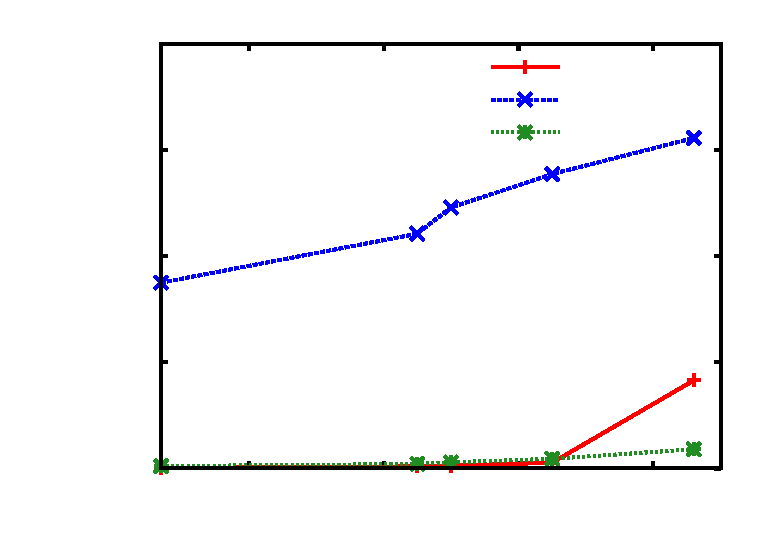
\includegraphics{proportions_phi}}%
    \gplfronttext
  \end{picture}%
\endgroup
}
	\caption{Proportion of the $10\%$ fastest particles amongst bond ordered particles. The jump in the proportion amongst \acs{MRCO} is only due to the poor statistics: at shallow supercooling the crystal-like particles are so few that the fast particles amongst them could not be detected.}
	\label{fig:proportions_phi}
\end{figure}

According to \citet{Berthier2007}, the structure cannot predict the dynamics at a local level. Thus, we decide to display in \FigureRef{fig:ordered_fast} only the the fast particles bonded to another fast particle and the icosahedra bonded to another icosahedra. The definition of the crystal-like particles is already taking into account the second shell, so we keep all \ac{MRCO} particles.

\begin{figure}
	\centering
	\begin{small}%
	\tikz\shade[ball color=green!33!black] circle (0.4em);
	Crystal-like\qquad%
	\tikz\shade[ball color=blue!33!black] circle (0.4em);
	Icosahedra\qquad%
	\tikz\shade[ball color=red] circle (0.4em);
	$10\%$ fastest\\
	\tikz\shade[ball color=yellow] circle (0.4em);
	$10\%$ fastest and crystal-like\\
	\tikz\shade[ball color=white] circle (0.4em);
	$10\%$ fastest and icosahedral%
	\end{small}\\
	\subfloat[Normal liquid ($\phi=0.479$)]{
		\label{fig:ordered_fast_liq}
		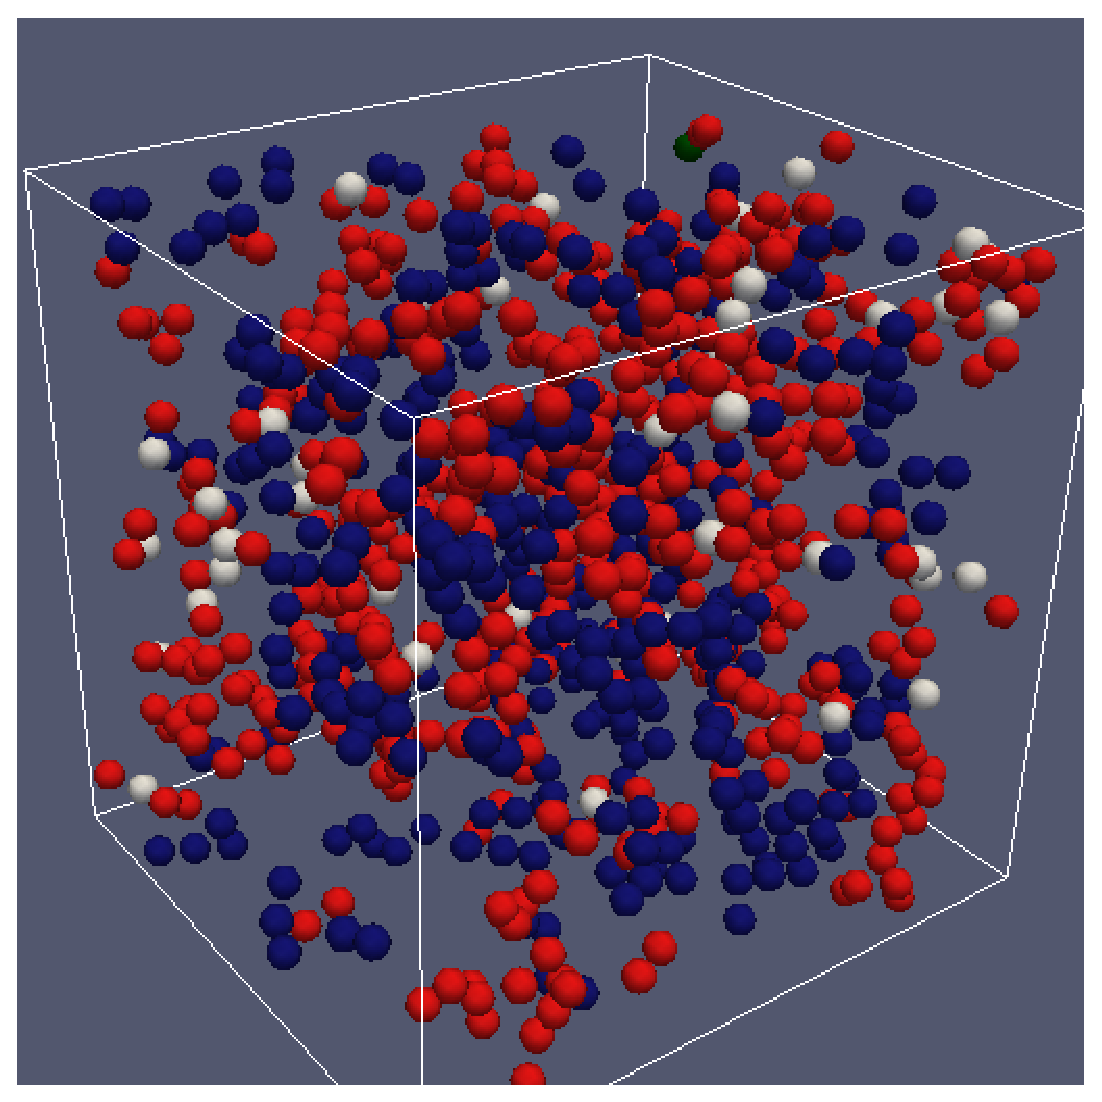
\includegraphics[width=0.4\textwidth]{ordered_fast_3954}}\quad
	\subfloat[Supercooled liquid ($\phi=0.535$)]{
		\label{fig:ordered_fast_sc}
		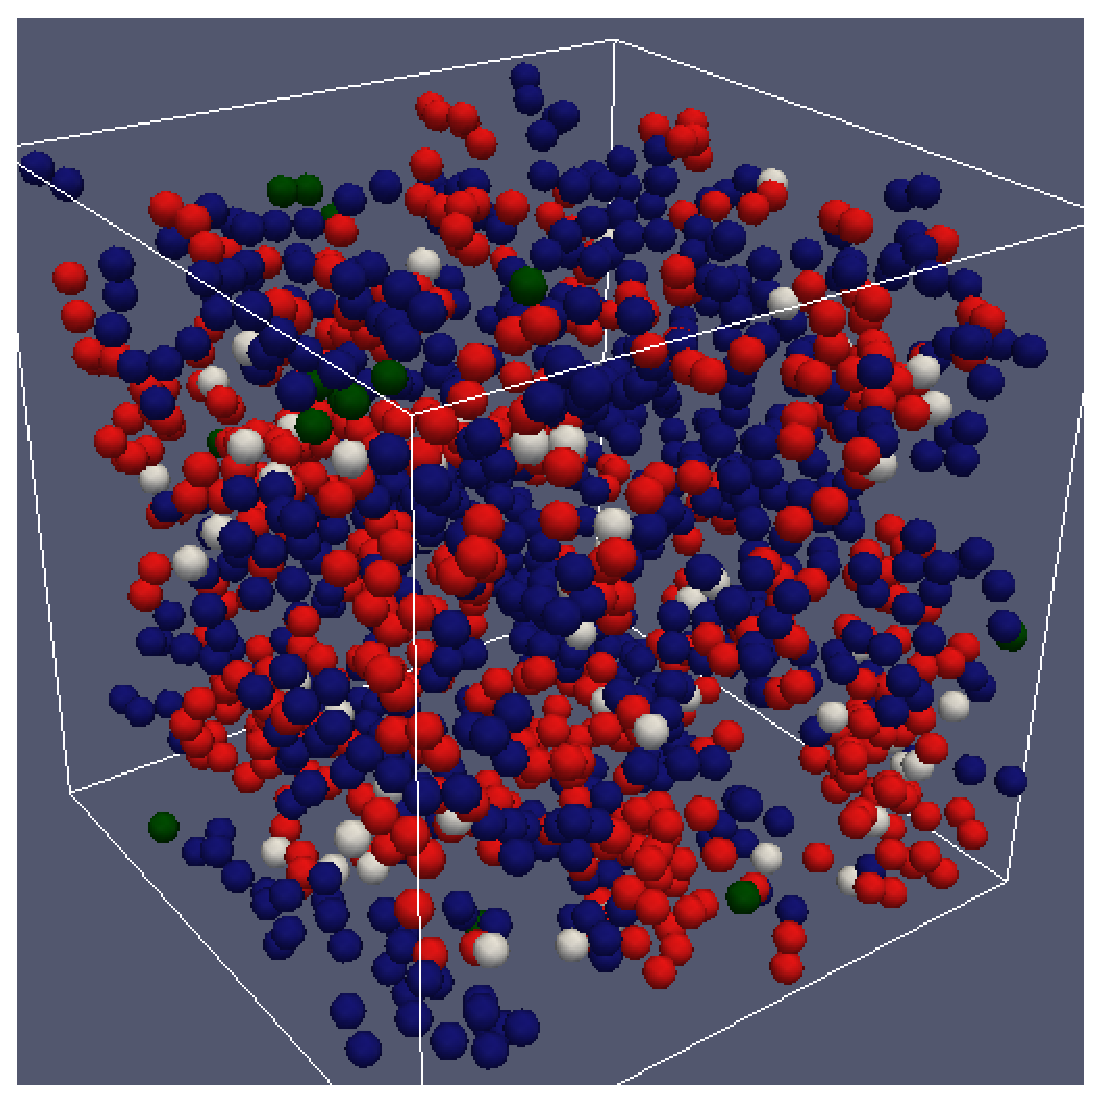
\includegraphics[width=0.4\textwidth]{ordered_fast_4582}}
	\caption{$10\%$ fastest particles and ordered particles.}
\end{figure}
\begin{figure}
	\ContinuedFloat
	\centering
	\begin{small}%
	\tikz\shade[ball color=green!33!black] circle (0.4em);
	Crystal-like\qquad%
	\tikz\shade[ball color=blue!33!black] circle (0.4em);
	Icosahedra\qquad%
	\tikz\shade[ball color=red] circle (0.4em);
	$10\%$ fastest\\
	\tikz\shade[ball color=yellow] circle (0.4em);
	$10\%$ fastest and crystal-like\\
	\tikz\shade[ball color=white] circle (0.4em);
	$10\%$ fastest and icosahedral%
	\end{small}\\
	\subfloat
		[Deeply supercooled ($\phi=0.576$). We are looking through a slice of the sample of thickness $\sim 8 \sigma$.]{
		\label{fig:ordered_fast_deep}
		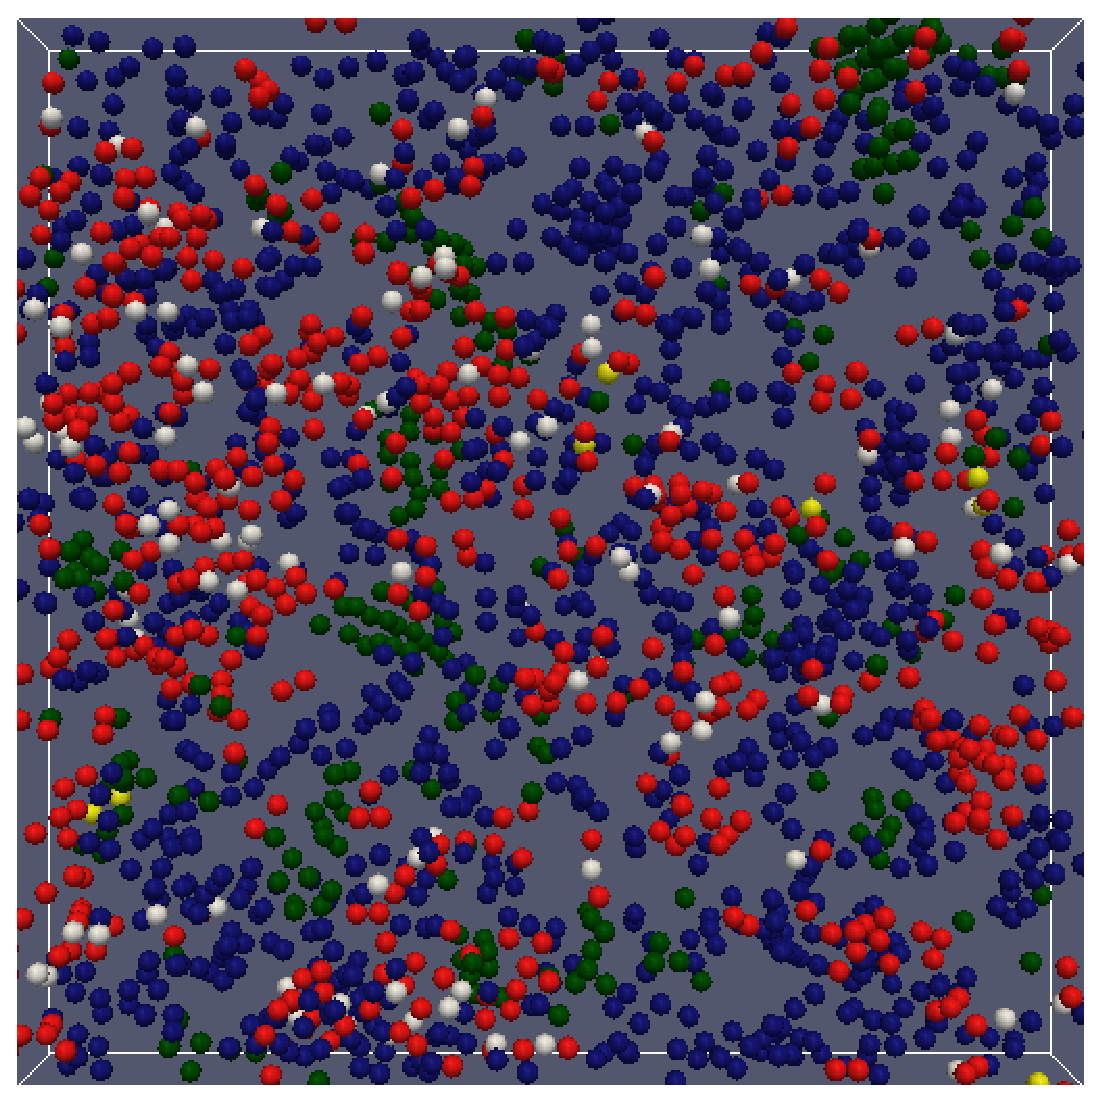
\includegraphics[width=0.8\textwidth]{ordered_fast_go1}}
	\caption{Icosahedra are in blue, crystal-like bond ordered particles in green and fast particles in red. Fast icosahedra are in white and fast \acs{MRCO} are in yellow if any.}
	\label{fig:ordered_fast}
\end{figure}

We observe that the position inside the icosahedral network influences the probability of having a fast particle: fast particles have preferentially one or two icosahedral neighbours, indicating that the ends and the arms of the network are more mobile than its junctions. This is reminiscent of the floppy modes in gels.

Overall, it seems that the icosahedral network do not play a direct role to prevent particle diffusion, whereas crystal-like order does.

\subsection{Bond order dynamic propensity}

In \SectionRef{sec:propensity} we presented the dynamic propensity invented by \citet{Widmer-Cooper2005} as a trick only accessible to simulations. However, we will present here a \emph{bond order dynamic propensity} that is accessible even in a system that cannot be restarted \latin{ad libitum} from the exact same overall configuration. This holds for all systems giving access to the coordinates where a sufficient ensemble average can be taken and - of course - where the bond orientational order plays a role.

The bond order propensity is defined as the ensemble average of the \ac{MSD} between $t_0$ and $t_0+t$ of all the particles that had the same structure at $t_0$. As explained in \ChapterRef{ch:structure}, the local structure of our system is well described by the $(w_6,Q_6)$-plane as in \FigureRef{fig:sc_w6Q6}, so we restrict the "same structure" condition to this plane:
\begin{equation}
	\mathcal{P}r(w_6, Q_6, t) \equiv \frac{
		\sum\limits_{t_0=0}^{t_{max}-t} \sum\limits_i{
			\left\|\vec{r_i}(t_0+t)-\vec{r_i}(t_0)\right\|^2 \delta(w_6^i-w_6) \delta(Q_6^i-Q_6)
			}
	}{
		\sum\limits_{t_0=0}^{t_{max}-t} \sum\limits_i{ \delta(w_6^i-w_6) \delta(Q_6^i-Q_6)}
	}
	\label{eq:bo_propensity}
\end{equation}
where the ensemble average is written as explicitly as possible. Because we average over all possible occurrences of a given $(w_6, Q_6)$ couple, all other possible causes of the dynamics are averaged down. The bond order propensity expresses the propensity for displacement of a given bond order.

\begin{figure}
	\centering
	\def\svgwidth{\textwidth}
	\input{msd_w6Q6quarter.pdf_tex}
	\caption{Bond order propensity in the $(w_6, Q_6)$ plane with increasing supercooling. For easier comparison, the propensity is normalised by the overall \acs{MSD}. The colour scale is saturated for $\mathcal{P}r>2\left\langle \Delta r^2\right\rangle$ to discard shot noise. All values are computed for the $t^{dh}$ of the sample. The population maps of \FigureRef{fig:sc_w6Q6} give an idea of the error bars.}
	\label{fig:msd_w6Q6}
\end{figure}

We plot the bond order propensity maps of our samples in \FigureRef{fig:msd_w6Q6}. We observe that for all volume fractions the propensity decreases along the $Q_6$ axis: crystal-like ordered particles are slower. The tendency is weak at low supercooling but dramatically develop when approaching the glass transition. This is coherent with what was found in 2D~\citep{kawasaki2007cbd, watanabe2008} but not yet confirmed in 3D.

A similar but weaker link between order and slowness is observed along the $w_6$ axis: icosahedral ordered particles are slower. However, the slowing down is significant only for $w_6<w_6^*$, \latin{i.e.} the almost perfect iscosahedra. This means that the free volume difference discussed in \SectionRef{sec:ico_volume} is linked to the stability of the icosahedra. We are able to differentiate between the stable icosahedra that slow down the system and the unstable ones that do not seem to have an effect on the dynamics.

The highest propensities are observed at high positive $w_6$ and when both $w_6$ and $Q_6$ are close to zero. However, these regions represent a very low population of particles (see \FigureRef{fig:sc_w6Q6}) so the signal to noise ratio is poor. The fact that few particles arrange in these structures may be related to their lack of stability. It would be then coherent that unstable structures present high propensity for motion.

\subsection{Summary}

The role of icosahedral ordering in the supercooled dynamics of hard spheres seems to be minor. Perfect icosahedra are indeed stable structures that prevent motion of their central particle. However, this effect remains local and does not extend to the distorted icosahedral network. Thus, the slowing down induced by icosahedral order do not grow in size approaching the glass transition.

The crystal-like bond ordered clusters proved to hinder the motion of their particles more than any other structure. This is especially true at deep supercooling when the characteristic size of the crystal-like bond order fluctuations grows, following the same law as the dynamic correlation length.
